\section{Classical Calculations}

\begin{frame}
\frametitle{Classical DFT Approach}
\begin{itemize}
    \item Periodic DFT calculations using CP2K
    \item System: Al(111) surface with triazole inhibitor
    \item Geometry optimization using ML potentials
\end{itemize}
\end{frame}

\begin{frame}
\frametitle{System Setup}
\begin{columns}
\column{0.5\textwidth}
\begin{itemize}
    \item 4×4 Al(111) supercell
    \item PBE functional with D3 dispersion correction
    \item DZVP-MOLOPT-GTH basis sets
\end{itemize}
\column{0.5\textwidth}
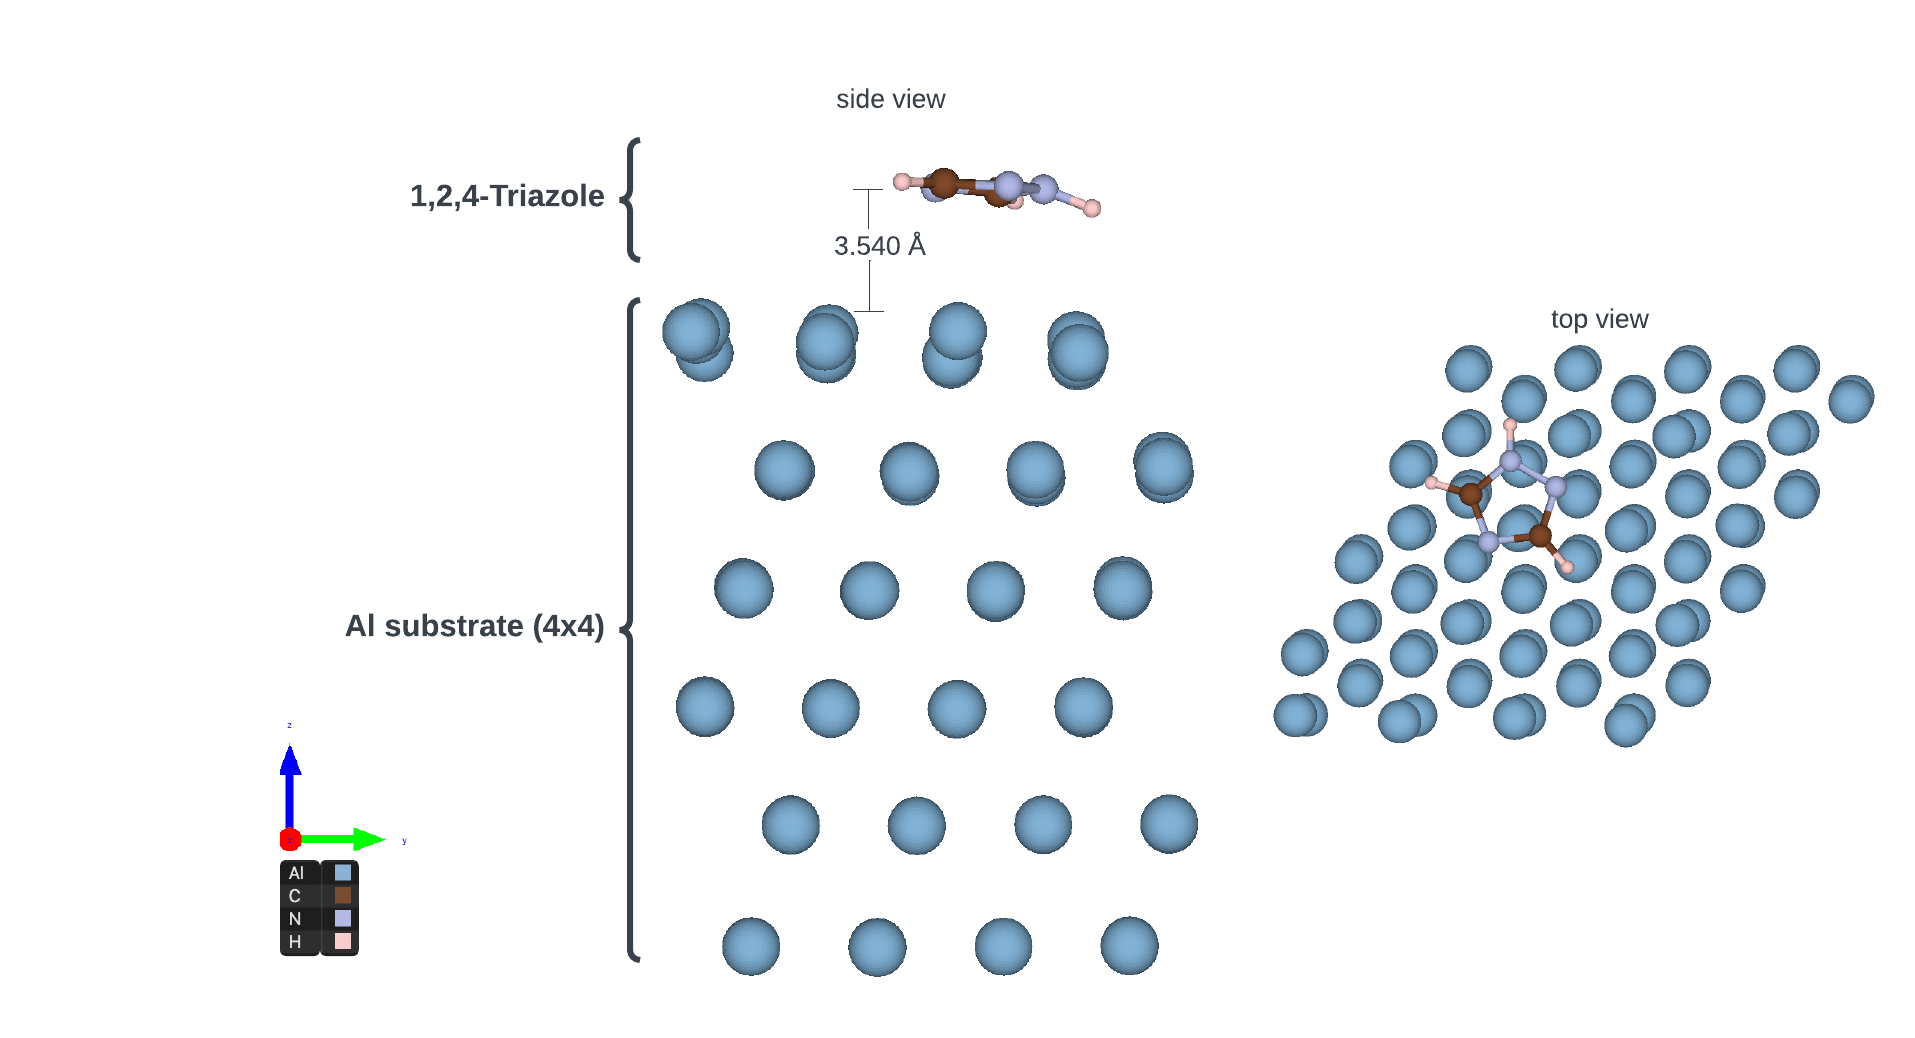
\includegraphics[width=\textwidth]{../../content/img/workflow_viz1.png}
\end{columns}
\end{frame}

\begin{frame}
\frametitle{System Description}
\begin{itemize}
    \item Optimized geometry of 1,2,4-triazole on Al(111)
    \item Periodic boundary conditions in XY plane
    \item Vacuum gap in Z direction
    \item Total system size: 8 atoms (inhibitor) + substrate
\end{itemize}
\end{frame} 